\documentclass{article}

% if you need to pass options to natbib, use, e.g.:
%     \PassOptionsToPackage{numbers, compress}{natbib}
% before loading neurips_2018

% ready for submission
% \usepackage{neurips_2018}

% to compile a preprint version, e.g., for submission to arXiv, add add the
% [preprint] option:
%     \usepackage[preprint]{neurips_2018}

% to compile a camera-ready version, add the [final] option, e.g.:
     \usepackage[final]{proposal}

% to avoid loading the natbib package, add option nonatbib:
% \usepackage[nonatbib]{proposal}

\usepackage[utf8]{inputenc} % allow utf-8 input
\usepackage[T1]{fontenc}    % use 8-bit T1 fonts
\usepackage{hyperref}       % hyperlinks
\usepackage{url}            % simple URL typesetting
\usepackage{booktabs}       % professional-quality tables
\usepackage{amsfonts}       % blackboard math symbols
\usepackage{nicefrac}       % compact symbols for 1/2, etc.
\usepackage{microtype}      % microtypography
\usepackage{fontspec, xunicode, xltxtra} 
\setmainfont{Microsoft YaHei} 
\setmainfont{Times New Roman}
\usepackage{ctex}


\title{《人工神经网络》大作业开题报告}

% The \author macro works with any number of authors. There are two commands
% used to separate the names and addresses of multiple authors: \And and \AND.
%
% Using \And between authors leaves it to LaTeX to determine where to break the
% lines. Using \AND forces a line break at that point. So, if LaTeX puts 3 of 4
% authors names on the first line, and the last on the second line, try using
% \AND instead of \And before the third author name.

\author{
  陶天骅\\
  计算机科学与技术系 \\
  清华大学 \\
  \texttt{tth17@mails.tsinghua.edu.cn} \\
  %% examples of more authors
  \AND
  杨雅儒\\
  计算机科学与技术系 \\
  清华大学 \\
  \texttt{yangyr17@mails.tinghua.edu.cn} \\
  %% \And
  %% Coauthor \\
  %% Affiliation \\
  %% Address \\
  %% \texttt{email} \\
}

\begin{document}
% \nipsfinalcopy is no longer used

\maketitle



\section{任务定义}

本课题希望构建一个神经网络以及一些简单的界面,可以根据用户提供的一些特征的比例,自动生成一张风景图片。程序界面示意图如下。

\begin{figure}[ht]
	\centering
	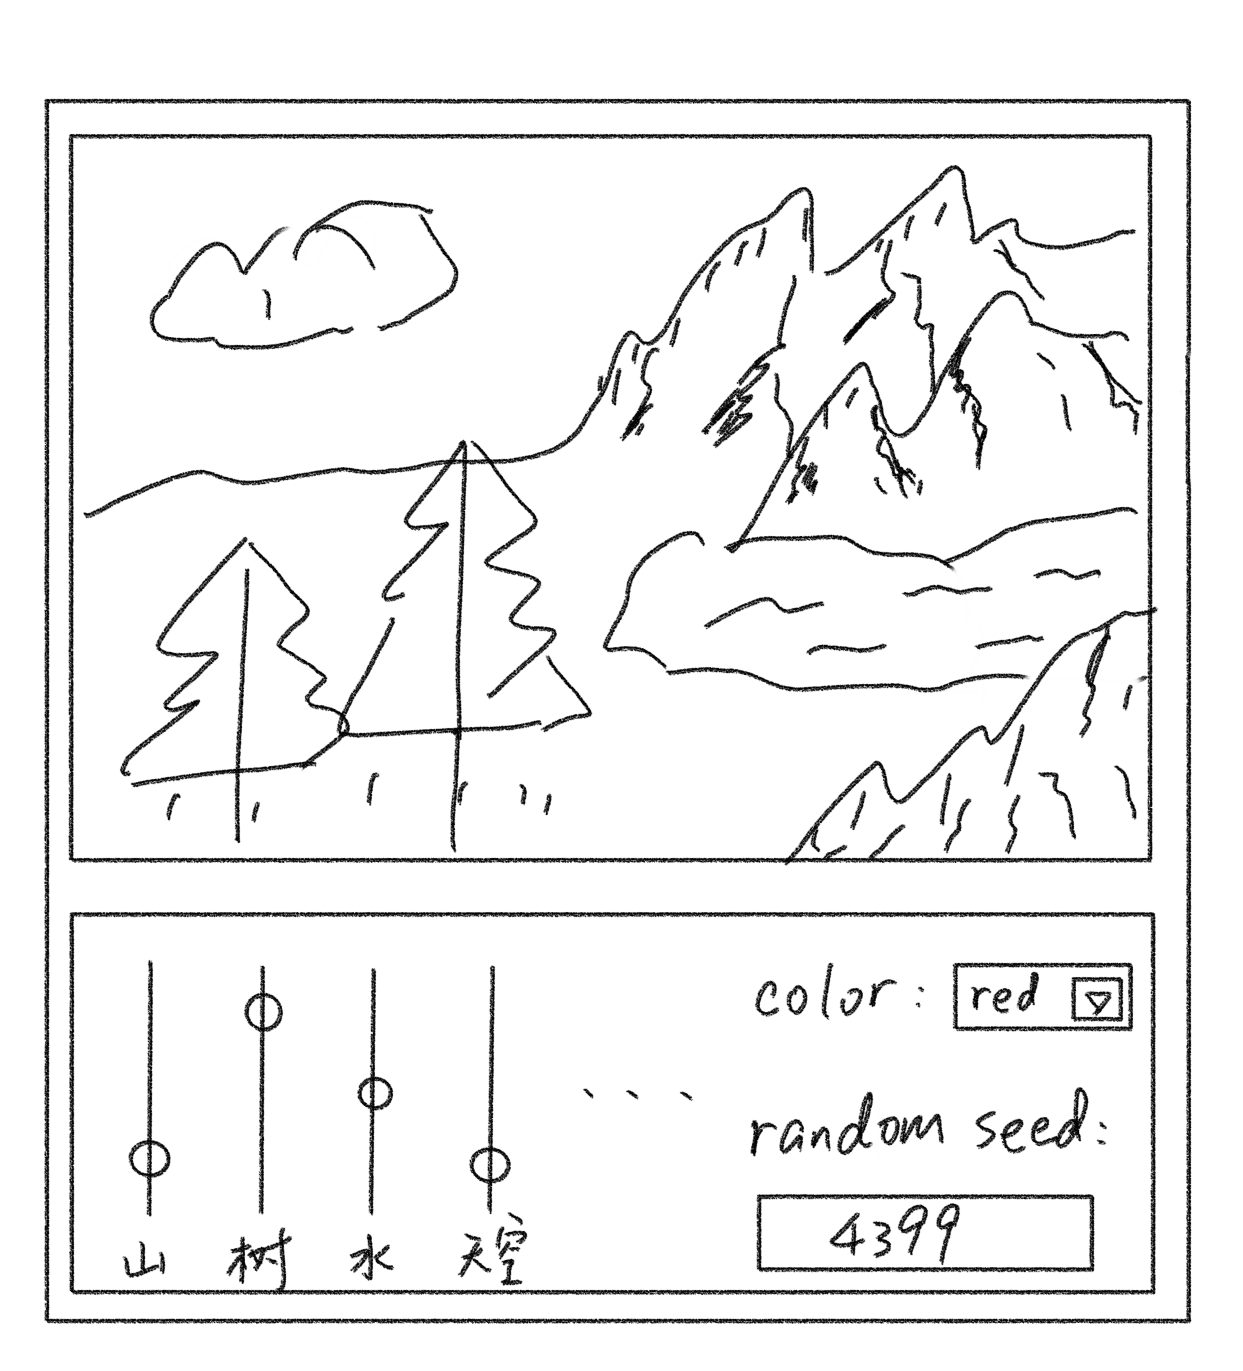
\includegraphics[scale=0.1]{res/sketch.png}
	\caption{A Simple Sketch.}
\end{figure}

用户通过滑动滑条,确定例如树木、山、水、天空等要素在图片中的占比,并可以设定希望使用的主题颜色,程序便生成一张符合以上要求的风景图片。用户可以设置随机种子来获得不同的图片。

用数学语言形式化程序的任务即为:

令 $pic$ 是一张图片,$label_{pic}$ 是图片的标签,值为 $real$ 或 $generated$ ,表示是真实的或者生成的。需要构建一个辨别器 $D$ ,参数是 $\theta_D$,$D(pic; \theta_D)$ 输出一个标签,表示辨别器认为 $pic$ 是否是生成的。训练目标为:

$$\mathop{\arg\max}_{\theta_D}(Prob(D(pic; \theta_D)=label_{pic}))$$

即$D$能给出正确的标签。

再构建生成器$G$,参数是$\theta_G$,对于一个特征向量$x$,$G(x; \theta_G)$输出一张图片。训练目标为:

$$\arg\min_{\theta_G}(Prob(D(G(x; \theta_G); \theta_D)=generated))$$

即$G$的输出应足够逼真,以至于$D$不能分辨图片是否是生成的。

同时为了让$G$能正确地展现$x$的特征,还需要一个编码器$E$,$E(pic)$输出图片对应的特征向量。$E$的训练就是AutoEncoder的$Encoder$的训练,而$decoder$的部分就是前面的$G$。当$E$是一个理想编码器的时候,$G$的训练目标还要包括:

$$\mathop{\arg\max}_{\theta_G}(Prob(E(G(x; theta_G))=x))$$

即对$G$在$x$上生成的图片进行编码的话,还能得到$x$,这表示生成的图片确实含有$x$的特征。


\section{数据集}

用于训练的数据集可以是从各大图片社交平台(如 Pinterest 、Flicker)上下载获得的风景图片。

\section{挑战和基线}

\subsection{挑战}
\begin{itemize}
	\item 确定使用哪些特征作为输入标签。
	\item 将特征和主题颜色向量化。
	\item 考虑到算力有限,可能无法生成分辨率较高的图片。
	\item 融合不同的神经网络架构,打造一个本程序专用的神经网络。
\end{itemize}

\subsection{基线}

\begin{itemize}

\item 基线1.
Nvidia的SPADE项目构建了一个程序,可以根据景物轮廓绘出风景图像,与本项目有类似之处,但是它使用了不同的原理。Nvidia的工作构造了一个称为GauGAN的网络,在COCO-Stuff, Cityscapes 和 ADE20K 数据集上学习了图像语义分割,再由特定类别的图像语义生成图像。
\item 基线2.

\end{itemize}

\section{研究计划}

\begin{enumerate}
	\item 收集训练数据
	\item 清洗数据
	\item 构建基于CNN、GAN、AutoEncoder的神经网络
	\item 构建GUI
	\item 训练
	\item 测试
\end{enumerate}

\section{可行性}
本项目使用到的主要方法为一些十分成熟的神经网络架构,主要难点在于将他们进行融合,并设计本项目专用的网络,因为既能保证可行性,又有创新点。在计算规模上,我们尽量将图片的大小控制在可以在单个GPU上训练的规模。
\end{document}
